% !TEX root = main.tex

% === ソフトウェア ==========================================================
\subsection{ソフトウェア構成}
本システムのソフトウェア構成について,以下に各要素を説明する.


% === 下位レイヤー ==========================================================
\subsubsection{下位レイヤー}
本システムの下位レイヤーソフトウェアでは,モーター制御,エンコーダーのデータ処理,
およびシリアル通信を実現するために自作ライブラリを使用している.
開発環境はCubeIDE(ver.1.16.1)である.
以下に,各ライブラリの詳細について説明する.

\paragraph{エンコーダーライブラリ (encoder.c, encoder.h)}\mbox{}\\
エンコーダーライブラリは,ロータリーエンコーダー(AMT102-V)の値を取得し,
角速度や回転数を計算するための機能をもつ.
このライブラリでは,エンコーダーから得られる値を高精度に利用するために4逓倍処理を行い,
モーターの速度制御に使用している.以下に,一部ライブラリコードを示す.


\lstset{language=C, caption={エンコーダーカウント値の取得}}

\begin{lstlisting}
    // エンコーダーカウント値の取得
    int Encoder_Read(Encoder* encoder)
    {
        int16_t count = (int16_t)(__HAL_TIM_GET_COUNTER(encoder->htim) - TIMER_MAX_COUNT / 2);
        return count;
    }
    
    void Encoder_Interrupt(Encoder* encoder, EncoderData* encoder_data)
    {
        int count = Encoder_Read(encoder);
    
        encoder_data->count = count;
        encoder_data->rot = count / (double)encoder->ppr;
        encoder_data->deg = encoder_data->rot * 360.0;
        encoder_data->distance = encoder_data->rot * (PI * encoder->diameter);
    
        encoder_data->rps = (encoder_data->rot - encoder->before_rot) / (encoder->period * 0.001);
        encoder_data->velocity = encoder_data->rps * PI * encoder->diameter;
    
        encoder->before_rot = encoder_data->rot;
    }
\end{lstlisting}

また,このライブラリではカウント値のリセット機能も提供しており,
特定の条件下でカウント値をゼロに戻すことが可能である.

\paragraph{モータードライバライブラリ (motor\_driver.c, motor\_driver.h)}\mbox{}\\
モータードライバライブラリは,DCモーターの速度と方向を制御するための機能をもつ.
このライブラリでは,PWM信号を用いてモーターを駆動し,
回転方向の切り替えや速度制御を行っていおる.
以下に,一部ライブラリコードを示す.

\lstset{language=C, caption=モーターの速度設定 (motor\_driver.c)}

\begin{lstlisting}
// 初期化関数
void MotorDriver_Init(MotorDriver* motor, TIM_HandleTypeDef* htimA, uint32_t channelA,TIM_HandleTypeDef* htimB, uint32_t channelB) {
motor->htimA = htimA;
motor->channelA = channelA;
motor->htimB = htimB;
motor->channelB = channelB;    
 // PWM 開始
HAL_TIM_PWM_Start(htimA, channelA);
HAL_TIM_PWM_Start(htimB, channelB);
}
// 速度設定関数
void MotorDriver_setSpeed(MotorDriver *motor, int speed) {
    int pwm_value;
    if (speed > 100) speed = 99;     //ブーストラップ回路に対応
    if (speed < -100) speed = -99;   //ブーストラップ回路に対応
        
    if (speed > 0) {
        pwm_value = (speed * __HAL_TIM_GET_AUTORELOAD(motor->htimA)) / 100;
        __HAL_TIM_SET_COMPARE(motor->htimA, motor->channelA, pwm_value);
        __HAL_TIM_SET_COMPARE(motor->htimB, motor->channelB, 0);
    } else {
        pwm_value = (-speed * __HAL_TIM_GET_AUTORELOAD(motor->htimA)) / 100;
        __HAL_TIM_SET_COMPARE(motor->htimA, motor->channelA, 0);
        __HAL_TIM_SET_COMPARE(motor->htimB, motor->channelB, pwm_value);
    }
}
\end{lstlisting}


\paragraph{シリアル通信ライブラリ (serial\_lib.c, serial\_lib.h)}\mbox{}\\
シリアル通信ライブラリは,PCや上位システムとのデータ通信を実現するために設計されている.
このライブラリでは,固定長および可変長データの送受信をサポートしており,
効率的かつ安全な通信を実現している.以下に,可変長データの送信および受信関数を示す.

\lstset{language=C, caption=可変長データの送受信関数 (serial\_lib.c)}

\begin{lstlisting}
// 可変長データの送信関数
void Serial_SendData(UART_HandleTypeDef *huart, int16_t *data, uint8_t data_count) {
    uint8_t buffer_size = 2 + data_count * 2;
    uint8_t *buffer = (uint8_t *)malloc(buffer_size);

    buffer[0] = SERIAL_HEADER1;
    buffer[1] = SERIAL_HEADER2;

    for (uint8_t i = 0; i < data_count; i++) {
        buffer[2 + i * 2] = (data[i] >> 8) & 0xFF;
        buffer[3 + i * 2] = data[i] & 0xFF;
    }

    HAL_UART_Transmit(huart, buffer, buffer_size, HAL_MAX_DELAY);
    free(buffer);
}
// 可変長データの受信関数
uint8_t Serial_ReceiveData(UART_HandleTypeDef *huart, int16_t *data, uint8_t data_count) {
    uint8_t buffer_size = 2 + data_count * 2;
    uint8_t *buffer = (uint8_t *)malloc(buffer_size);

    if (HAL_UART_Receive(huart, buffer, buffer_size, HAL_MAX_DELAY) == HAL_OK) {
        if (buffer[0] == SERIAL_HEADER1 && buffer[1] == SERIAL_HEADER2) {
            for (uint8_t i = 0; i < data_count; i++) {
                data[i] = (buffer[2 + i * 2] << 8) | buffer[3 + i * 2];
            }
            free(buffer);
            return 1; // 正常受信
        }
    }
    free(buffer);
    return 0; // エラー
}
\end{lstlisting}

この関数では,データを指定された形式に従ってパケット化し,
シリアル通信で送信する.
先頭にヘッダー(`SERIAL\_HEADER1` と `SERIAL\_HEADER2`)を追加し,
データ部分は16ビット整数をビッグエンディアン形式で格納する.
また,送信後に動的に確保したメモリを解放することで,メモリリークを防止している.

受信関数では,指定された形式に従って受信したデータをデコードし,
データバッファに格納する.受信データのヘッダーを検証し,
データが正しい形式であることを確認した後,各データを16ビット整数として復元する.
受信データが無効の場合,エラーコードを返すことで通信エラーを適切にハンドリングする.


\paragraph{メインコード (main.c)}\mbox{}\\
メインコードでは,自作のエンコーダー,モータードライバ,シリアル通信ライブラリを統合し,
システム全体の制御を実現している.
このコードは,PCからの制御信号を受信してモーターの速度を設定するとともに,
エンコーダーから取得した速度データをPCに送信する役割を果たす.

この制御ループでは,まずシリアル通信ライブラリの`Serial\_ReceiveData`関数を使用して
PCからの制御信号を受信する.受信した制御信号は右車輪および左車輪の目標速度を表しており,
それぞれ`controlSignalRight`と`controlSignalLeft`に格納される.
これらの速度データは,モータードライバライブラリの`MotorDriver\_setSpeed`関数を用いて
設定される.

次に,エンコーダーデータの送信を行う.10msごとにタイマーの値を確認し,
タイミングが来た場合にエンコーダーライブラリの`Encoder\_Interrupt`関数を使用して
速度データを更新する.更新された速度データは,
シリアル通信ライブラリの`Serial\_SendData`関数を用いてPCに送信される.

このように,メインコードは上位システムとの通信,モーター制御,
およびエンコーダーデータの送信を連携させ,ロボット全体のリアルタイム制御を実現している.


以下に,一部実装コードを示す.

\lstset{language=C, caption=メイン制御ループ (main.c)}
\begin{lstlisting}
// メイン制御ループ
while (1)
{
    /* PC からの制御信号を受信 */
    int16_t receivedData[2];
    if (Serial_ReceiveData(&huart2, receivedData, 2))
    {
        controlSignalRight = receivedData[0];
        controlSignalLeft = receivedData[1];

        MotorDriver_setSpeed(&motorRight, -1 * controlSignalRight);
        MotorDriver_setSpeed(&motorLeft, -1 * controlSignalLeft);
    }

    /* エンコーダーデータの送信( 10[ms] ごとに送信) */
    if (HAL_GetTick() - lastSendTime >= 10)
    {
        lastSendTime = HAL_GetTick();

        /* エンコーダーの速度データを更新 */
        Encoder_Interrupt(&encoderRight, &encoderDataRight);
        Encoder_Interrupt(&encoderLeft, &encoderDataLeft);

        /* エンコーダー速度を送信 */
        int16_t feedbackData[2] = {(int16_t)encoderDataRight.velocity, (int16_t)encoderDataLeft.velocity};
        Serial_SendData(&huart2, feedbackData, 2);
    }
}
\end{lstlisting}


% === 上位レイヤー ==========================================================
\subsubsection{上位レイヤー}
本システムの上位レイヤーでは,以下のROS2ノードを利用してリアルタイムなデータ処理と通信を実現している.
開発環境はROS2 humble ,Python 3.10.12 である.

本研究で使用したROS2ノードは以下の通りである.
\begin{itemize}
    \item \textbf{web\_socket\_node}: Webブラウザと通信し,ロボットに指令を与える.
    \item \textbf{PID\_node}: PID制御を用いてモーター制御信号を生成.
    \item \textbf{RealSense\_node}: 深度カメラからデータを取得し,ターゲットの位置を推定.
    \item \textbf{serial\_read\_node}: 下位レイヤーとのシリアル通信を通じてエンコーダーデータを受信.
    \item \textbf{serial\_send\_node}: モーター制御信号を下位レイヤーに送信.
    \item \textbf{Roboware\_node}: ロボット全体の管理,および追従アルゴリズムを搭載.
\end{itemize}

図\ref{fig:rqt}にrqt\_graphによりノード間の接続状況を視覚化したものを示す.

\begin{figure}[H]
    \centering
    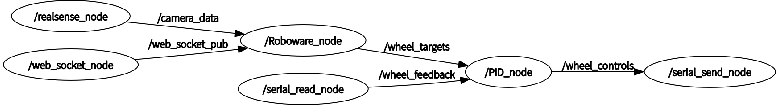
\includegraphics[width=1.0\textwidth]{figure/rqtgraph_v1.4.pdf}
    \caption{rqtgraph}
    \label{fig:rqt}
\end{figure}


\paragraph{web\_socket\_node}\mbox{}\\
web\_socket\_nodeは,FastAPIを使用してWebブラウザとROS2ノード間の双方向通信を行う.
Webブラウザからはロボットの制御指令を送信でき,ロボットの現在位置や状態をリアルタイムで取得できる.

FastAPIは軽量かつ高性能なWebフレームワークであり,非同期通信をサポートするため,
WebSocketを用いたリアルタイム通信にも対応している.
WebSocketは、HTTPプロトコルを拡張した双方向通信のためのプロトコルであり,効率的なデータ送受信を可能にする.

\begin{itemize}
    \item \textbf{購読トピック}
          \begin{itemize}
              \item \texttt{estimated\_position} (\texttt{Float32MultiArray}): 推定位置データ
          \end{itemize}
    \item \textbf{発行トピック}
          \begin{itemize}
              \item \texttt{web\_socket\_pub} (\texttt{String}): WebSocket通信で受信したコマンド
          \end{itemize}
\end{itemize}


以下に,WebSocket通信の主要な実装部分を示す.

\begin{lstlisting}[language=Python, caption=WebSocket通信の主要部分 (web\_socket\_node.py)]
# FastAPI インスタンスの作成
app = FastAPI()

# WebSocket 通信のエンドポイント
@app.websocket('/ws')
async def websocket_endpoint(websocket: FastAPIWebSocket):
    await websocket.accept()
    try:
        while True:
            # クライアントからのデータを受信
            receive_data = await websocket.receive_text()
            
            # ROS トピックにデータをパブリッシュ
            msg = String()
            msg.data = receive_data
            self.pub.publish(msg)

            # サブスクライブしたデータをクライアントに送信
            string_send_data = ",".join(map(str, self.send_data))
            await websocket.send_text(string_send_data)
    except Exception as e:
        print(f'WebSocket error: {str(e)}')
    finally:
        print('WebSocket disconnected')
\end{lstlisting}

この実装では,Webブラウザから送信された制御信号をROSトピック`web\_socket\_pub`にパブリッシュし,
ROS2ノードで処理される.
同時に,ROS2ノードがサブスクライブしたデータをWebブラウザに送信することでリアルタイム通信を実現している.


\paragraph{PID\_node}\mbox{}\\
PID\_nodeは,ロボットのモーター制御信号を生成するためにPID制御アルゴリズムを実装したノードである.
PID制御では,目標値と現在値の差(偏差)を基に比例(P),積分(I),微分(D)の3要素を組み合わせて制御信号を生成する.
さらに,本ノードでは微分項にローパスフィルタを適用し,ノイズの影響を低減している.

本ノードは以下のROSトピックを使用する.
\begin{itemize}
    \item \textbf{購読トピック}
          \begin{itemize}
              \item \texttt{wheel\_targets} (\texttt{Float32MultiArray}): 目標速度データ(右車輪,左車輪)
              \item \texttt{wheel\_feedback} (\texttt{Float32MultiArray}): 現在速度データ(右車輪,左車輪)
          \end{itemize}
    \item \textbf{発行トピック}
          \begin{itemize}
              \item \texttt{wheel\_controls} (\texttt{Float32MultiArray}): 制御信号(右車輪,左車輪)
          \end{itemize}
\end{itemize}

以下に,PID制御アルゴリズムの主要な実装部分を示す.

\begin{lstlisting}[language=Python, caption=PID制御アルゴリズムの実装 (PID\_node.py)]
class PIDController:
    def __init__(self, kp, ki, kd, tau=0.01):
        self.kp = kp
        self.ki = ki
        self.kd = kd
        self.tau = tau  # ローパスフィルタの時定数
        self.prev_error = 0.0
        self.integral = 0.0
        self.prev_derivative = 0.0  # 前回の微分値

    def compute(self, target, current, dt):
        error = target - current
        self.integral += error * dt

        # 微分項にローパスフィルタを適用
        raw_derivative = (error - self.prev_error) / dt
        derivative = (self.tau * self.prev_derivative + dt * raw_derivative) / (self.tau + dt)
        self.prev_derivative = derivative
        self.prev_error = error

        return self.kp * error + self.ki * self.integral + self.kd * derivative
\end{lstlisting}

このアルゴリズムでは,目標速度と現在速度の差を計算し,PID制御の各要素を基に制御信号を生成する.
ローパスフィルタを導入することで,ノイズによる微分項の影響を抑制し,安定した制御信号を生成する.

次に,制御ループの主要部分を以下に示す.

\begin{lstlisting}[language=Python, caption=制御ループ (PID\_node.py)]
def control_loop(self):
    current_time = self.get_clock().now()
    dt = (current_time - self.last_time).nanoseconds / 1e9
    self.last_time = current_time

    # 右車輪と左車輪の制御信号を計算
    control_signal_right = self.pid_right.compute(self.target_right, self.current_right, dt)
    control_signal_left = self.pid_left.compute(self.target_left, self.current_left, dt)

    # 制御信号をパブリッシュ
    control_msg = Float32MultiArray()
    control_msg.data = [float(control_signal_right), float(control_signal_left)]
    self.pub.publish(control_msg)
\end{lstlisting}

この制御ループでは,以下の手順でモーター制御信号を生成する.
\begin{enumerate}
    \item 目標速度と現在速度の偏差を計算し,PID制御を実行.
    \item 生成した制御信号をROSトピック\texttt{wheel\_controls}にパブリッシュ.
    \item デバッグ用に制御信号の詳細をログ出力.
\end{enumerate}

これにより,ロボットの速度を目標値に追従させるためのリアルタイム制御が可能となる.


\paragraph{RealSense\_node}\mbox{}\\
RealSense\_nodeは,Intel RealSense D435iカメラを使用して深度データとRGB画像を処理し,ターゲットの検出および距離・オフセット情報を生成する.このノードは,YOLOv5を利用した物体検出アルゴリズムを実装しており,人物の位置と距離をリアルタイムで推定してパブリッシュする.

本ノードは以下のROSトピックを使用する.
\begin{itemize}
    \item \textbf{発行トピック}
          \begin{itemize}
              \item \texttt{camera\_data} (\texttt{Float32MultiArray}): 人物の距離とオフセット情報
          \end{itemize}
\end{itemize}

以下に,主要な処理と実装部分を示す.

\begin{lstlisting}[language=Python, caption=ターゲット検出と距離推定 (RealSense\_node.py)]
# RealSense フレームの処理
def process_frames(self):
    try:
        frames = self.pipeline.wait_for_frames()
        depth_frame = frames.get_depth_frame()
        color_frame = frames.get_color_frame()
        if not depth_frame or not color_frame:
            return

        # 深度データとRGB データを取得
        depth_image = np.asanyarray(depth_frame.get_data())
        color_image = np.asanyarray(color_frame.get_data())

        # YOLOv5 による物体検出
        results = self.model(color_image)
        for result in results.xyxy[0]:  # 検出結果をループ
            box, conf, cls = result[:4], result[4], int(result[5])
            if cls == 0:  # クラス0(人物)のみ処理
                x1, y1, x2, y2 = map(int, box)
                center_x, center_y = (x1 + x2) // 2, (y1 + y2) // 2

                # 深度データから距離とオフセットを計算
                raw_distance = depth_frame.get_distance(center_x, center_y)
                offset_x = center_x - (color_image.shape[1] // 2)
                filtered_distance = self.filter_distance(raw_distance)

                # データをパブリッシュ
                msg = Float32MultiArray()
                msg.data = [filtered_distance, float(offset_x)]
                self.publisher.publish(msg)

                # デバッグ情報の表示
                self.get_logger().info(
                    f"Published camera data: Distance={filtered_distance:.2f}, Offset={offset_x}"
                )
                break
    except Exception as e:
        self.get_logger().error(f"Error processing frames: {str(e)}")
\end{lstlisting}

距離データは,近づく場合はそのままの値を使用し,遠ざかる場合は移動平均フィルタを適用している.
このフィルタリングは,測定誤差やノイズの影響を低減するためである.

\begin{lstlisting}[language=Python, caption=距離データのフィルタリング (RealSense\_node.py)]
def filter_distance(self, current_distance):
    if current_distance == 0.0:  # 無効値は無視
        return self.previous_distance

    if current_distance < self.previous_distance:
        # 近づいている場合: そのままの値を使用
        self.distance_history = [current_distance]  # 履歴をリセット
        return current_distance
    else:
        # 遠ざかる場合: 移動平均フィルタを適用
        self.distance_history.append(current_distance)
        if len(self.distance_history) > self.history_size:
            self.distance_history.pop(0)  # 古い値を削除
        return sum(self.distance_history) / len(self.distance_history)
\end{lstlisting}

本ノードは,RealSenseカメラから取得した深度データとRGB画像をもとに,
YOLOv5を用いたターゲット検出と距離推定を行い,リアルタイムでROSトピックに結果をパブリッシュする.

\paragraph{serial\_read\_node}\mbox{}\\
serial\_read\_nodeは,下位レイヤーから送信されるエンコーダーデータをシリアル通信を通じて受信し,
ROSトピックにパブリッシュする役割を持つ.
このノードは非同期通信をサポートしており,リアルタイムでのデータ受信とパブリッシュを実現している.

\begin{itemize}
    \item \textbf{発行トピック}
          \begin{itemize}
              \item \texttt{wheel\_feedback} (\texttt{Float32MultiArray}): エンコーダーデータ(右車輪,左車輪)
          \end{itemize}
\end{itemize}

以下に,主要なコード部分を示す.

\begin{lstlisting}[language=Python, caption=シリアルデータの受信とトピックへのパブリッシュ (serial\_read\_node.py)]
class SerialReadNode(Node):
    def __init__(self):
        super().__init__('serial_read_node')
        self.publisher = self.create_publisher(Float32MultiArray, 'wheel_feedback', 10)
        # シリアル通信の設定
        self.serial_port = serial.Serial('/dev/ttyUSB0', 115200, timeout=1)
        self.create_timer(0.1, self.read_serial_data)
    def read_serial_data(self):
        try:
            if self.serial_port.in_waiting > 0:
                data = self.serial_port.read(8)  # 8バイトを読み取る
                right_speed, left_speed = struct.unpack('>hh', data[2:])  # データのデコード
                msg = Float32MultiArray()
                msg.data = [float(right_speed), float(left_speed)]
                self.publisher.publish(msg)
                self.get_logger().info(f"Published wheel_feedback: {msg.data}")
        except Exception as e:
            self.get_logger().error(f"Error reading serial data: {str(e)}")
\end{lstlisting}

このノードでは,シリアルポートから受信したエンコーダーデータを解析し,
右車輪と左車輪の速度データとしてトピック\texttt{wheel\_feedback}にパブリッシュする.

\paragraph{serial\_send\_node}\mbox{}\\
serial\_send\_nodeは,上位レイヤーからのモーター制御信号を下位レイヤーに送信する役割を持つ.
このノードは,ROSトピックから制御信号を受け取り,指定されたフォーマットで
パケット化してシリアル通信を通じて下位レイヤーに送信する.

\begin{itemize}
    \item \textbf{購読トピック}
          \begin{itemize}
              \item \texttt{wheel\_controls} (\texttt{Float32MultiArray}): モーター制御信号(右車輪,左車輪)
          \end{itemize}
\end{itemize}

以下に,主要なコード部分を示す.

\begin{lstlisting}[language=Python, caption=制御信号の送信 (serial\_send\_node.py)]
class SerialSendNode(Node):
    def __init__(self):
        super().__init__('serial_send_node')
        self.subscription = self.create_subscription(
            Float32MultiArray,
            'wheel_controls',
            self.send_serial_data,
            10
        )
        # シリアル通信の設定
        self.serial_port = serial.Serial('/dev/ttyUSB0', 115200, timeout=1)
    def send_serial_data(self, msg):
        try:
            if len(msg.data) == 2:
                right_control, left_control = int(msg.data[0]), int(msg.data[1])
                data = struct.pack('>BBhh', 0xA5, 0xA5, right_control, left_control)
                self.serial_port.write(data)
                self.get_logger().info(f"Sent wheel_controls: {msg.data}")
        except Exception as e:
            self.get_logger().error(f"Error sending serial data: {str(e)}")
\end{lstlisting}

このノードでは,モーター制御信号をROSトピック\texttt{wheel\_controls}から受信し,
指定されたフォーマットでパケット化してシリアル通信を通じて送信する.


\paragraph{Roboware\_node}\mbox{}\\
Roboware\_nodeは,ロボットの速度制御を実現するためのノードであり,
比例航法 (PN),修正比例航法 (MPN),およびゲインスケジューリング下修正比例航法 (GS-MPN)
をサポートしている.
これらのアルゴリズムを用いて,ターゲットを追従する速度と角速度を計算し,
逆運動学を用いて車輪ごとの目標速度を決定する.

\begin{itemize}
    \item \textbf{購読トピック}
          \begin{itemize}
              \item \texttt{web\_socket\_pub} (\texttt{String}): 操作モードおよびロボット制御信号
              \item \texttt{camera\_data} (\texttt{Float32MultiArray}): 距離とオフセットデータ
          \end{itemize}
    \item \textbf{発行トピック}
          \begin{itemize}
              \item \texttt{wheel\_targets} (\texttt{Float32MultiArray}): 車輪ごとの目標速度
          \end{itemize}
\end{itemize}

以下に,各アルゴリズムでの速度計算部分を示す.

\subparagraph{PN (Proportional Navigation)}\mbox{}\\
PNアルゴリズムでは,以下のように直進速度$V$と角速度$\omega$を計算する.
\begin{lstlisting}[language=Python, caption=PNの計算部分 (Roboware\_node\_np.py)]
V = self.kp_v * (self.person_distance - 1.0)
omega = (self.navigation_constant) * self.kp_omega * self.person_offset / max((self.person_distance), 1.0)
\end{lstlisting}

\subparagraph{MPN (Modified Proportional Navigation)}\mbox{}\\
MPNでは,偏差角速度の微分を用いて動作をなめらかにするため,以下のように計算する.
\begin{lstlisting}[language=Python, caption=MPNの計算部分 (Roboware\_node\_mpn.py)]
offset_rate = (self.person_offset - self.previous_offset) / self.dt  # 偏差角速度
V = self.kp_v * (self.person_distance - 1.0)
omega = (
    self.navigation_constant * self.kp_omega * self.person_offset / self.person_distance +
    self.lambda_gain * offset_rate
)
self.previous_offset = self.person_offset  # 偏差を更新
\end{lstlisting}

\subparagraph{GS-MPN (Gain-Scheduled Modified Proportional Navigation)}\mbox{}\\
GS-MPNでは,動的微分ゲインを導入し,偏差角速度に基づく調整を行う.
\begin{lstlisting}[language=Python, caption=GS-MPNの計算部分 (Roboware\_node\_newmpn.py)]
offset_rate = (self.person_offset - self.previous_offset) / self.dt  # 偏差角速度
dynamic_kd = self.kd_lambda * (1 - math.exp(-self.a * abs(offset_rate))) / (1 + math.exp(-self.a * abs(offset_rate)))
V = self.kp_v * (self.person_distance - 1.0)
omega = (
    self.navigation_constant * self.kp_omega * self.person_offset / self.person_distance +
    dynamic_kd * offset_rate
)
self.previous_offset = self.person_offset  # 偏差を更新
\end{lstlisting}


また,カメラからの座標変換も行っている.
\begin{lstlisting}[language=Python, caption=座標変換]
def position_callback(self, msg):
    if len(msg.data) == 2:  
        pixel_offset = msg.data[1]  # カメラ画像上の水平ズレ(ピクセル)
        depth = msg.data[0]  # カメラから取得した深度値( m )
        # 座標変換
        x_camera = (pixel_offset * depth) / self.fx  # カメラ座標系のX
        y_camera = depth  # カメラ座標系のY

        # ロボット座標系への変換
        x_robot = x_camera + self.camera_offset_x
        y_robot = y_camera

        # 更新
        self.person_offset = x_robot  # ロボット座標系のX
        self.person_distance = y_robot  # ロボット座標系のY
\end{lstlisting}

本ノードでは,各種追従アルゴリズムを動的に選択できるよう設計されており,追従性能の向上と滑らかな動作を実現している.
また,逆運動学を用いることで,車輪ごとの速度制御信号を正確に生成する.
